\documentclass{article}
\usepackage{algpseudocode}
\usepackage{listings}
\usepackage{amsmath}
\usepackage{graphicx}

\title{Java Random seed searching by state prediction and bit lifting}
\author{by Kris}
\date{July 2024}

\begin{document}
\maketitle

\section{Introduction}
Work in progress.\\
Seed searching is the process of finding initial seeds of a pseudo-random number generator (PRNG) that satisfy a specific set of conditions.
This document is intended to be a practical reference guide to two advanced seed searching techniques: bit lifting and state prediction, in the context of Minecraft seed finding and/or seed cracking.

\section{An overview of Java Random}
In this section, we will briefly discuss the Java Random PRNG and its key functions.

To generate pseudo-random numbers, Java Random internally stores a 48-bit integer, called the (internal) state, or (internal) seed of the generator. The internal state is not directly accessible by the generator’s user. Every time the user requests a pseudo-random number from the PRNG, that state is updated, potentially multiple times, and some function of the new state(s) is returned to as the output. The state update (advancement) function, \Call{nextSeed}{}, is defined as follows:

\
\begin{algorithmic}
\Function{nextSeed}{} 
    \State $state \gets (state \times M + A)$ mod $2^{48}$
\EndFunction
\end{algorithmic}
\ \

\noindent Where $a$ mod $b$ denotes an operator that returns the positive remainder from dividing $a$ by $b$, and $M, A$ are constant integers. For the sake of completeness:
\begin{equation}\notag
    M = 25214903917, \quad A = 11
\end{equation}
\ \

This type of pseudo-random number generation algorithm is called a Linear Congruential Generator (LCG). The values of $M$ and $A$ are chosen in such a way that the \Call{nextSeed}{} function always cycles through all $2^{48}$ possible states before returning to the same state. (todo: citation needed)

The \Call{nextSeed}{} function on its own is not enough to create a self-sufficient PRNG. The second key function of Java Random is \Call{setSeed}{$seed$}, which is used to set the internal state of the generator using a user-provided seed as follows:

\
\begin{algorithmic}
\Function{setSeed}{$seed$} 
    \State $state \gets (seed \oplus M)$ mod $2^{48}$
\EndFunction
\end{algorithmic}
\ \

\noindent where $M$ is the same constant integer as in \Call{nextSeed}{}, and $\oplus$ is the XOR operator.

It’s worth noting that this effectively gives the user the ability to set the internal state to an arbitrary number of their choice, $n$, by simply calling \Call{setSeed}{$n \oplus M$}. The point of this function is to allow the user to be able to deterministically reproduce a sequence of pseudo-random numbers. This is extremely useful in situations like Minecraft’s world generation, where the player expects to get the exact same world by inputting the exact same world seed, while the world itself still appears “random”.\\
The third key function of Java Random is \Call{next}{$numBits$}, defined as follows:

\
\begin{algorithmic}
\Function{next}{$numBits$} 
    \State \Call{nextSeed}{}
    \State \Return $state \gg (48 - numBits)$
\EndFunction
\end{algorithmic}
\ \

\noindent which first advances the internal state of the generator, then returns the top $numBits$ bits of the new state as an integer. It serves as a helper for more complex operations.

\indent Java Random contains a small set of specialized functions that the user can call to get a specific type of random number. In Minecraft, the most frequently used ones are: \Call{nextInt}{$bound$}, \Call{nextFloat}{}, and \Call{nextLong}{}. 
The source code, along with detailed comments for all of the functions can be found in Appendix A. %REF!
In order to understand state prediction and bit lifting, being familiar with their implementations is strongly recommended (todo: link to java.util.Random documentation).

\section{Multiple-state and backwards advancement}

In seed searching practice, it’s often necessary to advance the internal state of Java Random multiple times in succession. Calling \Call{nextSeed}{} in a loop is a simple, but inefficient solution. Fortunately, there exists a way to quickly calculate the parameters of a multiple-state advancement function, \Call{advanceByN}{}, for an arbitrarily large $N$.

Let’s find a function that advances the internal state of Java Random by 2, by substituting \Call{nextSeed}{} as the state for another \Call{nextSeed}{}:

\begin{algorithmic}
\Function{advance2}{} 
    \State $state \gets (((state \times M + A)$ mod $2^{48}) \times M + A)$ mod $2^{48}$
\EndFunction
\end{algorithmic}
\ \

\noindent We can omit the first mod $2^{48}$, since the expression is taken mod $2^{48}$ at the end anyway. By distributing the multiplication over the terms in parenthesis, we get

\
\begin{algorithmic}
\Function{advanceBy2}{} 
    \State $state \gets (state \times M^2 + M \times A + A)$ mod $2^{48}$
\EndFunction
\end{algorithmic}
\ \

\noindent $M^2$ and $M \times A + A$ are both constants, let’s call them $M_2$, $A_2$.

\
\begin{algorithmic}
\Function{advanceBy2}{} 
    \State $state \gets (state \times M_2 + A_2)$ mod $2^{48}$
\EndFunction
\end{algorithmic}
\ \

We could combine two \Call{advanceBy2}{} calls into \Call{advanceBy4}{}, then two \Call{advanceBy4}{} into \Call{advanceBy8}{}, and so on. This way, it’s possible to advance the state by any power of two. That, in turn, gives us the ability to advance the state $n$ times by combining appropriate power-of-two advancement functions for each bit that’s set to true in the binary representation of $n$.
As an example, to find a function that advances the state by 14, which is 1110 in binary, we can combine \Call{advanceBy8}{}, \Call{advanceBy4}{}, and \Call{advanceBy2}{}. 
We can also find a function that calculates the previous state of Java Random. Because an advancement by $2^{48}$ would make the generator return to the same state, an advancement by $2^{48}-1$ would be equivalent to “going back” by 1 state in the generator. \\
By precalculating the parameters of a particular \Call{advanceByN}{} function, we can achieve performance similar to a single \Call{nextSeed}{} call, which is paramount to efficient seed searching.

\section{State prediction}

State prediction is one of the most crucial seed searching techniques. It aims to exploit the simplicity of Java Random’s functions, most commonly \Call{nextInt}{$bound$} and \Call{nextFloat}{}, to predict which values of the internal state could have been mapped to a known pseudo-random number. In this section, we will present the general idea behind state prediction for \Call{nextInt}{$bound$} and \Call{nextFloat}{}, providing examples of practical applications.

\subsection{ nextInt($bound$) }

Let’s assume for now that $bound$ is a power of two. In that case, the function simplifies to

\
\begin{algorithmic}
\Function{nextInt}{$bound$} 
    \State \Return $(bound \times \Call{next}{31} \gg 31$
\EndFunction
\end{algorithmic}
\ \

\noindent expanding the \Call{next}{31},

\
\begin{algorithmic}
\Function{nextInt}{$bound$}
    \State \Call{nextSeed}{}
    \State \Return $(bound \times (state \gg 17)) \gg 31$
\EndFunction
\end{algorithmic}
\ \

\noindent Since $n$ is a power of 2, we can replace the multiplication by a left-side bit-shift of the right-hand-side by $log_2(n)$ bits:

\
\begin{algorithmic}
\Function{nextInt}{$bound$}
    \State \Call{nextSeed}{}
    \State \Return $((state \gg 17) \ll log_2(bound)) \gg 31$
\EndFunction
\end{algorithmic}
\ \

\noindent Cleaning up the bit-shifts,

\
\begin{algorithmic}
\Function{nextInt}{$bound$}
    \State \Call{nextSeed}{}
    \State \Return $state \gg (48 - log_2(bound))$
\EndFunction
\end{algorithmic}
\ \

After advancing the internal state, the function returns the topmost \\$log_2(bound)$ bits as the result. If we know that a call to \Call{nextInt}{$bound$} returned $r$, we could approach this from a different angle. Since the return value of the function was $r$, and $bound$ is a power of two, then the top $log_2(bound)$ bits of the generator’s state after calling \Call{nextInt}{$bound$} must have been numerically equal to $r$. \\
Let’s look at an example of how this can speed up seed searching. Suppose that we know that a Java Random PRNG with a particular starting state generated the following numbers in a given sequence of calls:

\begin{algorithmic}
    \State $\Call{nextInt}{4} \to 3$
    \State $\Call{nextInt}{4} \to 0$
    \State $\Call{nextInt}{16} \to 9$
    \State $\Call{nextInt}{8} \to 2$\\
\end{algorithmic}

\noindent Although checking all $2^{48}$ starting internal states is possible, we can apply state prediction for the first call, \Call{nextInt}{4}, and simply set the top 2 bits of the state to 3, or 11 in binary, and check the remaining $2^{46}$ possibilities of lower 46 bit values. 
Even better, if we state-predict using the \Call{nextInt}{16} call instead, then filter the value of \Call{nextInt}{8}, go back 3 states using a precalculated state advancement function, and filter the two \Call{nextInt}{4} values, we will only need to check $2^{44}$ possibilities, one sixteenth of the full range of $2^{48}$ state values. %TODO A Java implementation of this example is available in Appendix C.1.

If the \Call{nextInt}{} bound is not a power of two, we can still apply state prediction, and it will be only slightly more complex. Simplifying the \Call{nextInt}{$bound$} function, we get

\
\begin{algorithmic}
\Function{nextInt}{$bound$}
    \State $bits \gets 0$
    \State $value \gets 0$
    \Repeat
        \State $bits = \Call{next}{31}$
        \State $value = bits$ mod $bound$
    \Until{$bits - value + bound - 1 >= 0$}
    \State \Return $value$
\EndFunction
\end{algorithmic}
\ \

Although the condition $bits - value + bound - 1 >= 0$ seems to be always true, the left-hand-side is treated as a 32-bit U2 signed integer (todo: citation needed), which means values greater than $2^{31} - 1$ will overflow and become negative. For small values of bound, we can ignore the loop, as it is very unlikely to run more than once (todo: further explanation). This approach is satisfactory for most practical applications. 
% TODO For how to handle cases where the loop would run more than once, see Appendix B. 

\
\begin{algorithmic}
\Function{nextInt}{$bound$}
    \State $bits = \Call{next}{31}$
    \State $value = bits$ mod $bound$
    \State \Return $value$
\EndFunction
\end{algorithmic}
\ \

\noindent Expanding the \Call{next}{31},

\
\begin{algorithmic}
\Function{nextInt}{$bound$}
    \Call{nextSeed}{}
    \State \Return $(state \gg 17)$ mod $bound$
\EndFunction
\end{algorithmic}
\ \

\noindent In this case, \Call{nextInt}{} advances the state by 1 and returns the top 31 bits of state modulo the bound.

\indent For a known \Call{nextInt}{} return value $r$, we can already predict that the upper 31 bits of the advanced state must have been of the form $\ a \times bound + r$. \\
Therefore, we can reduce the search space of possible states by a factor of $bound$:

\begin{algorithmic}
\State $upper \gets r$
\While{$upper < 2^{31}$}
    \For{$lower \gets 0..2^{17}-1$}
        \State $state \gets (upper \ll 17) \ | \ lower$
        \Comment{"$|$" being the bitwise OR operator}
        \State ...
        \Comment{Check the remaining conditions}
    \EndFor
    \State $upper \gets upper + bound$
    \Comment{The remainder mod $bound$ is unchanged}
\EndWhile
\end{algorithmic}
\ \

Let’s take a look at a very practical example of state prediction for \Call{nextInt}{} with a non-power of two bound. Suppose that we have the following conditions on an unknown 48-bit integer $s$, where $P, Q, R$ are known integer constants:

\
\begin{algorithmic}
\State $\Call{setSeed}{s + R}$
\State $\Call{nextInt}{23} \to 0$
\State $\Call{nextInt}{23} \to 0$
\State $\Call{setSeed}{s - P + R}$
\State $\Call{nextInt}{23} \to 22$
\State $\Call{nextInt}{23} \to 0$
\State $\Call{setSeed}{s - Q + R}$
\State $\Call{nextInt}{23} \to 0$
\State $\Call{nextInt}{23} \to 22$
\State $\Call{setSeed}{s - P - Q + R}$
\State $\Call{nextInt}{23} \to 22$
\State $\Call{nextInt}{23} \to 22$
\end{algorithmic}
\ \

We will ignore for now what these conditions represent, and focus on how to find values of s that satisfy them efficiently. All \Call{nextInt}{} bounds here are 23, so we can state-predict any of the calls and check the remaining ones. Let’s choose the first \Call{nextInt}{23} after \Call{setSeed}{$s + R$} to be our state-predicted call. From there, we can filter the next condition, $\Call{nextInt}{23} \to 0$, and go back 2 states to retrieve the state right after \Call{setSeed}{$s + R$}, which we'll call $state_0$ (notice that we're ignoring the unlikely possibility that any of the two \Call{nextInt}{23} calls might have caused more than one state advancement).\\
We have
\begin{align*}
    & state_0 = (s + R) \oplus M \\
    & state_0 \oplus M = s + R \\
    & s = (state_0 \oplus M) - R
\end{align*}

and since the values of $state_0, M, R$ are all known, we can retrieve $s$ using the last equation, at which point checking the remaining conditions is simple. We have obtained an algorithm for finding Minecraft seeds that have a cluster of 4 nether structures spawning in minimal proximity from each other at 0,0. Further explanation of this example is available in Appendix B. %REF! 
%TODO A simple Java implementation of this example and a link to a CUDA kernel are available in Appendix C.2.

%TODO B: \Call{nextFloat}{} state prediction
\subsection{ nextFloat() }

\Call{nextInt}{$bound$} is not the only type of call that we can apply state prediction for. We can also easily deduce the possible states for a given range of \Call{nextFloat}{} return values by looking at the implementation of the function:

\
\begin{algorithmic}
\Function{nextFloat}{}
\State $\Return \frac{\Call{next}{24}}{1 \ll 24}$
\EndFunction
\end{algorithmic}
\ \

\noindent Expanding the \Call{next}{24},

\
\begin{algorithmic}
\Function{nextFloat}{}
\State \Call{nextSeed}{}
\State $\Return \frac{state \gg 24}{1 \ll 24}$
\EndFunction
\end{algorithmic}
\ \

\noindent The top 24 bits of $state$ can have a value of at most $2^{24} - 1$, therefore the division by $2^{24}$ maps that integer value to a fraction in the range [0, 1), or, more specifically,
[0, $1 - \frac{1}{2^{24}}$]. Each fractional \Call{nextFloat}{} return value can easily be mapped back to a corresponding integer value of the state's top 24 bits by multiplying the fraction by $2^{24}$. 
Even better, we can map entire ranges of fractions to ranges of integers, simply by multiplying both extremes by $2^{24}$. The only slight complication we need to consider is when the extremes of a known range of \Call{nextFloat}{} return values aren't integer multiples of $\frac{1}{2^{24}}$. We can handle this by rounding the result of the multiplication of such an extreme by $2^{24}$ to the nearest smaller integer for the range's maximum, and to the nearest greater integer for the minimum. 
The equation for mapping a fractional range to a range of 24-bit values can therefore be written as

\begin{equation}
    (bits_{min}, \ bits_{max}) = \left( \left\lceil frac_{min} \times 2^{24} \right\rceil, \left\lfloor frac_{max} \times 2^{24} \right\rfloor \right)
\end{equation}

Finally, let's look at a general example of how this equation can be utilized to reduce the search space of internal states:

\
\begin{algorithmic}
\State $upper \gets bits_{min}$
\While{$upper \le bits_{max}$}
    \For{$lower \gets 0..2^{24}-1$}
        \State $state \gets (upper \ll 24) | lower$
        \Comment{"$|$" being the bitwise OR operator}
        \State ...
        \Comment{Check the remaining conditions}
    \EndFor
    \State $upper \gets upper + 1$
\EndWhile
\end{algorithmic}
\ \

\section{Bit lifting}

Bit lifting is an advanced seed searching technique which utilizes weaknesses of the Java Random PRNG. Due to a lack of comprehensive resources and an in-depth explanation, it confuses many beginners and even experts. In this section, we will break down the basic concepts behind bit lifting and see how it can be used in practical scenarios.

\subsection{Shortened-state LCGs}

Consider the following three, similar Linear Congruential Generators:

\
\begin{algorithmic}
    \State $state \gets (6 \times state + 7)$ mod 1000
    \Comment{LCG$_1$}
    \State $state \gets (6 \times state + 7)$ mod 100
    \Comment{LCG$_2$}
    \State $state \gets (6 \times state + 7)$ mod 10
    \Comment{LCG$_3$}
\end{algorithmic}
\ \

\noindent Starting from $state = 0$, let’s list the next couple of consecutive states for all three LCGs:

\begin{table}[h]
    \centering
    \begin{tabular}{|c|c|c|}
    \hline
         LCG$_1$ state & LCG$_2$ state & LCG$_3$ state \\
    \hline
         0 & 0 & 0   \\
         7 & 7 & 7   \\
         49 & 49 & 9  \\
         301 & 1 & 1   \\
         813 & 13 & 3  \\
         885 & 85 & 5  \\
    \hline
    \end{tabular}
    \caption{Consecutive states for LCG$_1$, LCG$_2$, and LCG$_3$}
    \label{tab:lcgs}
\end{table}

Notice that the last digits of consecutive state triplets are equal. The moduli, 1000, 100 and 10, are powers of ten, so they simply cut off excessive decimal digits without affecting the entire state. Because of that, it’s impossible for the upper digits of a state to affect the lower digits of future states. It’s best to visualize this property with the help of an example. Consider a state of the form [ $upper$ ][ $lower$ ] where $upper$ and $lower$ represent sequences of decimal digits. We can represent this state as the following sum:
\begin{equation}
    upper \times 10^k + lower
\end{equation}
\noindent with $k$ being the amount of digits in $lower$. If we were to multiply this state by any integer, it would take the form
\begin{equation}
    n \times upper \times 10^k + n \times lower
\end{equation}
\noindent As the multiplication by $10^k$ is still there, the value of $upper$ did not affect the new $k$ lower digits. This statement holds true when we take the whole expression mod $10^m$, as that could only cut off the lower digits when all the upper digits were already cut off.

Most importantly, a similar property is satisfied for binary states. Because the LCG inside Java Random uses a modulus of $2^{48}$, at the end of a state update, any binary digits (bits) above the 48-th get cut off without affecting the entire state. Therefore, the upper bits of a Java Random state do not affect the lower bits of any future state. This is the core idea that makes bit lifting possible.

Since the lower bits in a Java Random state are not affected by the more significant bits, we can consider shortened-state LCGs that have the same multiplier and addend as Java Random but a smaller modulus, $2^m$. Such LCGs will follow the exact same cycle of states as the lower $m$ bits of the full-state Java Random. For $m = 1$, we would get the LCG
\begin{algorithmic}
    \State $state \gets (state \times M + A)$ mod 2
\end{algorithmic}
\noindent and since the Java Random constants $M, A$ are both odd,
\begin{algorithmic}
    \State $state \gets (state + 1)$ mod 2
\end{algorithmic}
\noindent That, in turn, implies that consecutive states of the full-state Java Random are of different parity.

\subsection{ Bit lifting using known values of nextInt($bound$) }

Bit lifting for \Call{nextInt}{$bound$} is only possible when the two following preconditions are met:
\begin{enumerate}
    \item $bound$ is even
    \item $bound$ is not a power of two
\end{enumerate}

\noindent Recall the simplified algorithm for \Call{nextInt}{$bound$} with the above conditions:

\
\begin{algorithmic}
\Function{nextInt}{$bound$}
    \Call{nextSeed}{}
    \State \Return $(state \gg 17)$ mod $bound$
\EndFunction
\end{algorithmic}
\ \

Let $s$ be the top 31 bits of the state after the \Call{nextSeed}{} call. Let us assume that we know the return value $r$ of the \Call{nextInt}{} call. Then,
\begin{equation}
    s \equiv r \quad (\text{mod} \ n)
\end{equation}

\noindent Therefore, there exists an integer $k$ such that
\begin{equation}\tag{$\star$}
     s = k \times n + r
\end{equation}

\noindent Let $p$ be the greatest integer power of two that divides $n$. Because $n$ is even, $p \ge 2$. Consider ($\star$) under mod $p$:

\begin{equation}
     s \equiv k \times n + r \quad (\text{mod} \ p)
\end{equation}

\noindent As $p \ | \ n$,

\begin{equation}\label{lifting.core}\tag{$\star\star$}
     s \equiv r \quad (\text{mod} \ p)
\end{equation}

Therefore, the $log_2(p)$ lower bits of s are numerically equal to $r$ mod $p$. We have lifted the middle bits of the internal state of Java Random using the return value of \Call{nextInt}{$bound$}. It is clear now why we needed $n$ to be an even number | otherwise we would not have any partial information about the middle bits.
Although this result might look extremely similar to what we achieved through state prediction for \Call{nextInt}{$2^n$}, in reality it is considerably more powerful.

The information we have obtained is bits 18 to $17 + log_2(p)$ of a Java Random internal state (counting from least to most significant bit, where the least significant bit is at index 1). We already know that those are independent from the more significant bits, so we can consider a shortened-state LCG with a modulus of $2^{17+log_2(p)}$. That gives us the ability to first rule out the lower bit values that don’t satisfy ($\star \star$), and then iterate the remaining upper bits to check the full conditions. This effectively reduces the search space by a factor of $p$, as checking the lower bit possibilities is usually much faster than the upper bit iteration phase. \\
By now we can address the first precondition of bit lifting | if $n$ was a power of two, we would only have information about the upper bits, so considering a shortened-state LCG would not be as beneficial. \\
Still, a reduction by a factor of $p$ is a worse outcome than we would expect from the simpler state prediction technique, so what is the point? Unlike state prediction, bit lifting can be applied with multiple conditions. Because the criteria of usage are also less restrictive (we don’t have a set formula for all seeds that satisfy the conditions), lifting is much more flexible and, as we will see, it can be applied in a number of obscure scenarios. 

Firstly, let’s look at a simplified example of bit lifting. We’re looking for integers $i$ that satisfy

\
\begin{algorithmic}
\State \Call{setSeed}{$i$}
\State $\Call{nextInt}{10} \to 1$
\State $\Call{nextInt}{12} \to 5$
\State $\Call{nextInt}{14} \to 0$
\State $\Call{nextInt}{16} \to 9$
\State $\Call{nextInt}{18} \to 2$
\State $\Call{nextInt}{20} \to 17$
\end{algorithmic}
\ \

Although it might be tempting to state-predict the \Call{nextInt}{20} and filter the remaining calls going backwards, let’s see how much information we can lift here. $10 = 2 \times 5$, which gives $log_2(2) = 1$ bits of information. $12 = 4 \times 3$, $log_2(4) = 2$ bits of information. Similarly, the \Call{nextInt}{14} call gives 1 bit, \Call{nextInt}{16} gives 0 since it does not satisfy the lifting preconditions, \Call{nextInt}{18} gives 1 bit and \Call{nextInt}{20} gives 2. In total, that’s 7 bits of information about the lower 20 bits of the potential state, which is a reduction by a factor of 128, more than 6 times the search space reduction achieved via state prediction. %TODO A Java implementation of this example can be found in Appendix C.3.

% \subsection{Practical applications of bit lifting}
% (structures, seedcrackerx)
% Having acquired some theoretical background, it's time to discuss ...

% \subsection{Iterative bit lifting}
% An interesting technique that can be used to gain ...

% \subsection{An unusual hybrid: bit lifting meets state prediction}
% In this final section on bit-lifting, we will ...

% consider adding this:
% \section{Hensel lifting}

\appendix

\section{An implementation of Java Random and frequently used functions}\label{appendix.jrand}

\begin{lstlisting}[language=Java]
public class JavaRandom {
    // The LCG's parameters:
    private static final long MULTIPLIER = 25214903917;
    private static final long ADDEND = 11;
    private static final long MODULUS = 1L << 48;
    // Instead of using the modulus itself, we can use
    // a bit mask on the lower 48 bits, which avoids
    // signed integer issues and is slightly faster
    private static final long MASK = MODULUS - 1;

    // state is a 48-bit integer, but internally
    // it's stored as a 64-bit long.
    private long state;

    public JavaRandom(long seed) {
        // Note the use of setSeed in the constructor.
        setSeed(seed);
    }

    public void setSeed(long seed) {
        state = (seed ^ MULTIPLIER) & MASK;
    }

    private void nextSeed() {
        state = (state * MULTIPLIER + ADDEND) & MASK;
    }

    // Notice that next(numBits) returns a 32-bit int, 
    // so it indirectly assumes numBits <= 32
    private int next(int numBits) {
        nextSeed();
        // >>> here is equivalent to the more natural,
        // arithmetic bit shift, >>, since state >= 0
        return (int)(state >>> 48-numBits);
    }

    // Returns a pseudo-random integer from the range
    // [0, bound-1]
    public int nextInt(int bound) {
        if(bound <= 0) {
            throw new IllegalArgumentException(
                "bound must be positive");
	}

        // Equivalent to "bound is a power of two"
        if((bound & -bound) == bound) {
            // Advance the state, then return the top 
            // log2(bound) bits. Casting next(31) to 
            // a long ensures that no overflow happens 
            // before we return the result.
            return (int)((bound * (long)next(31)) >> 31);
	}
 
        int bits = 0, value = 0;
        do {
            // Advance the state and take the top 31 bits
            bits = next(31);
            value = bits % bound;
        } while(bits - value + (bound - 1) < 0);
        // The condition is only true if an integer 
        // overflow happened
        
        return value;
    }

    public float nextFloat() {
        // Advance the state and take the top 24 bits, 
        // then map that value to a uniformly distributed 
        // fraction in the range [0, 1)
        return next(24) / ((float)(1 << 24));
    }

    public long nextLong() {
        // Take two upper 32-bit values from consecutive 
        // states and sum them together, moving the first 
        // value up by 32 bits. Note that next(32) returns
        // a signed value.
        return ((long)(next(32)) << 32) + next(32);
    }
}
\end{lstlisting}

\section{Minecraft region structure generation}\label{appendix.regionstructures}

In this section, we will explore one specific aspect of Minecraft's world generation | region structures.
As the name "region structures" suggests, they are a special type of structure which generates in what's called a region. Inside one region, there can only be one region structure of a given type.\\
Each region structure can be described as a set of 3 integer parameters: $spacing$, $separation$, and $salt$. The first parameter, $spacing$ determines how many chunks the regions for a given structure span. For example, the spacing for Desert Temples is 32 chunks, or 512 blocks, which means that Desert Temple regions are areas of 512 by 512 blocks on the $X$ and $Z$ axes. \\

\begin{figure}[htbp]
    \centering
    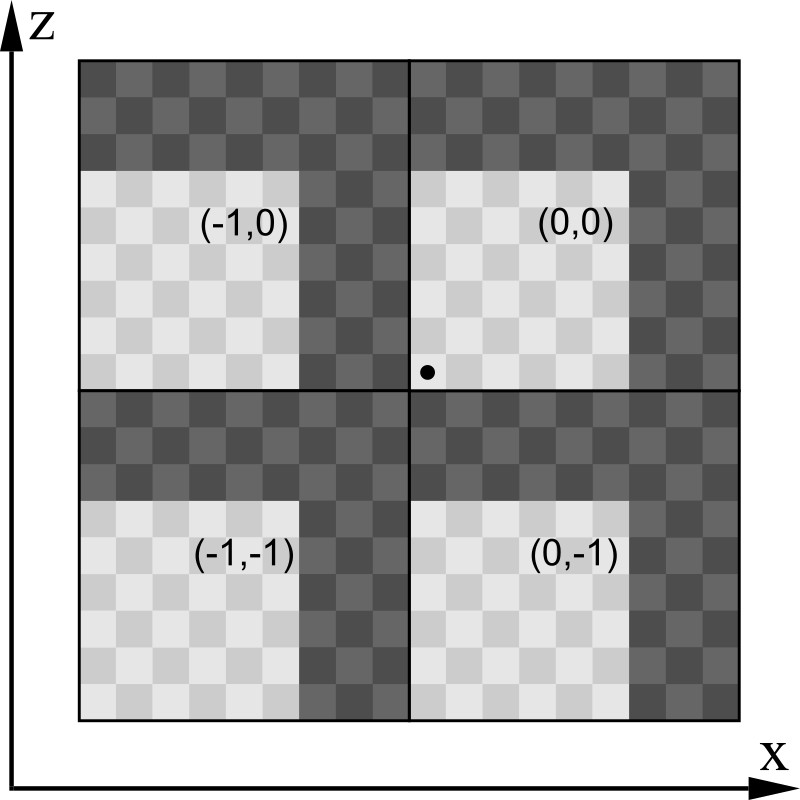
\includegraphics[width=0.5\linewidth]{regions.png}
    \caption{Regions around the world coordinates $(0,0)$ for $spacing = 9, \ separation = 3$. The small, shaded squares represent individual chunks. The dot indicates chunk (0,0).}
    \label{fig:regions}
\end{figure}

All regions are placed in a grid-like pattern, right next to each other, with no spaces in between, in the entire Minecraft world. Each region's position is linked with a pair of region coordinates, $(x_r, z_r)$. For a given block position and region spacing, we can calculate the region position of the region inside which the block is located as
\begin{equation}
    (x_r, z_r) = \left( \left\lfloor \frac{x_{block}}{16 \times spacing} \right\rfloor,\ \left\lfloor \frac{z_{block}}{16 \times spacing} \right\rfloor \right)
\end{equation}

\noindent Similarly, for a given chunk position,
\begin{equation}
    (x_r, z_r) = \left( \left\lfloor \frac{x_{chunk}}{spacing} \right\rfloor,\ \left\lfloor \frac{z_{chunk}}{spacing} \right\rfloor \right)
\end{equation}

The second parameter, $separation$, is the minimum distance between two region structures' starting chunk positions. It effectively creates a padding area, where the region structure can't start generating, around each region's upper borders (the borders with the maximum $x$ or $z$ coordinate), as illustrated in Figure 1. %REF!

The third parameter, salt, influences how an instance of Java Random responsible for the generation of a region structure's position is seeded. 
Let's examine how all three of these parameters combined are used to determine the chunk position of a region structure for region coordinates $(x_r, z_r)$ and a known world seed $w$:

\
\begin{algorithmic}
\State \Call{setSeed}{$w + P \times x_r + Q \times z_r + salt$}
\State $x_{chunk} \gets x_r \times spacing + \Call{nextInt}{spacing - separation}$
\State $z_{chunk} \gets z_r \times spacing + \Call{nextInt}{spacing - separation}$
\end{algorithmic}
\ \

\noindent For clarity, the values of $P, Q$ are known integer constants:
\begin{equation}\notag
    P = 341873128712, \quad Q = 132897987541
\end{equation}

As we can see, the algorithm first seeds a Java Random PRNG using the world seed, region position and $salt$. This ensures that different regions use different sequences of pseudo-random numbers to generate a given region structure. As $salt$ is different for different region structures, even if two region structures had the same $spacing$ and $separation$, their positions inside a specific region would not be the same in most cases. The Minecraft world seed, $w$, is a 64-bit number, but since Java Random operates under mod $2^{48}$, only the lower 48 bits of the seed are used by the algorithm. This is why the lower 48 bits of the world seed are often called the \emph{structure seed}. \\
The expressions $x_r \times spacing$ and $z_r \times spacing$ denote the minimum chunk position inside the region $x_r, z_r$, while $\Call{nextInt}{spacing - separation}$ offsets the generated chunk position by a pseudo-random value between 0 and $spacing - separation - 1$ inclusive.

The values of $spacing, separation, salt$ for a specific region structure and a specific version of Minecraft can be found inside the version's jar file, under 
\begin{verbatim} data/minecraft/worldgen/structure_set \end{verbatim}
\end{document}
